\documentclass{article}
\newcommand{\final}{0}
% Change to 1 for final submission, all notes are suppressed

\usepackage[final]{template}
\usepackage[utf8]{inputenc} % allow utf-8 input
\usepackage[T1]{fontenc}    % use 8-bit T1 fonts
\usepackage{hyperref}       % hyperlinks
\usepackage{url}            % simple URL typesetting
\usepackage{booktabs}       % professional-quality tables
\usepackage{amsfonts}       % blackboard math symbols
\usepackage{nicefrac}       % compact symbols for 1/2, etc.
\usepackage{microtype}      % microtypography
\usepackage{epsfig}
\usepackage{color}
\usepackage{parskip}
\usepackage{ifthen}
\usepackage{float}
\usepackage{alltt}
\usepackage{amsmath}
\usepackage{amssymb}
\usepackage{amsthm}
\usepackage{newlfont} % for Box
\usepackage{floatflt}
\usepackage{wrapfig}
\usepackage{fixltx2e}
\usepackage{subcaption} % for subfloat
\usepackage{multirow}
%\usepackage[breaklinks=true,bookmarks=false]{hyperref}
\usepackage{cleveref}
\usepackage{algorithmic}
\usepackage[export]{adjustbox}
\usepackage{mathtools, cuted}
%\usepackage[ruled]{algorithm2e} % For algorithms
\usepackage{microtype}
\usepackage{graphicx}
\usepackage{hyperref}

% Attempt to make hyperref and algorithmic work together better:
\newcommand{\theHalgorithm}{\arabic{algorithm}}

\newcommand*\samethanks[1][\value{footnote}]{\footnotemark[#1]}
\def\textrightarrow{$\rightarrow$}
\newcommand{\pcline }{\rule{0in}{0.0in}    }  % Spacing for pseudo-code.
\newcommand{\pctab  }{\hspace{0.10in}      }  % Pseudo-code indentation.
\newcommand{\pcbigtab  }{\hspace{1.75in}    }  % Pseudo-code indentation.
\newcommand{\pcasgn }{\mbox{$\leftarrow$}  }  % Pseudo-code assignment operator
\newcommand{\pcomment}[1]{\mbox{// {\it #1}}}  % Pseudo-code comments.
\newcommand{\pckeyword}[1]{\mbox{{\bf #1}}}  % Pseudo-code keywords.
\newcommand{\pcspace}{\hspace{0.10in}}

\newcommand{\pcode}[1]{
    \footnotesize
    \vspace{-0.1in}
    \begin{minipage}{100in} % The width argument will be ignored:
                            % See lamport p. 99
    \begin{tabbing} \hspace{0.10in} \= \pctab \= \pctab \= \pctab \= \pcbigtab \= \\
        #1
    \end{tabbing}
    \end{minipage}
%    \vspace{0.15in}
    }
%
\renewcommand{\algorithmicrequire}{\textbf{Input:}}
\renewcommand{\algorithmicensure}{\textbf{Output:}}

\newcommand{\tabtextsize}{\small}
\newcommand{\figtext}[1]{{\footnotesize #1}}
\newcommand{\Caption}[2]{\caption[#1]{{\em #1} #2}}
\newcommand{\invisible}[1]{{\color{white} #1}}
\newcommand{\emacsquote}[1]{{``#1''}}

\definecolor{color1}{rgb}{0.7,0,0}
\definecolor{color2}{rgb}{0,0.4,0}
\definecolor{color3}{rgb}{0,0,0.8}
\newcommand{\zjy}[1]{{\color{color1} Jiayao Zhang: #1 $\qed$}}
\newcommand{\szh}[1]{{\color{color2} Zehao Su: #1 $\qed$}}
\newcommand{\lc}[1]{{\color{color3} Chen Liu: #1 $\qed$}}
\newcommand{\warning}[1]{{\it\color{red} #1}}
\newcommand{\note}[1]{{\it\color{blue} #1}}
\newcommand{\nothing}[1]{}
\newcommand{\passthrough}[1]{#1}
\definecolor{AudioColor}{rgb}{0.56,0.34,0.62}
\newcommand{\audio}[1]{{\color{AudioColor} Audio: #1}}

\newcommand{\psdraftboxDefault}{\psnodraftbox}

\definecolor{figred}{rgb}{1,0,0}
\definecolor{figgreen}{rgb}{0,0.6,0}
\definecolor{figblue}{rgb}{0,0,1}
\definecolor{figpink}{rgb}{1,0.63,0.63}

%\ifthenelse{\equal{\final}{1}}
%{
%\renewcommand{\zjy}[1]{}
%\renewcommand{\szh}[1]{}
%\renewcommand{\lc}[1]{}
%\renewcommand{\warning}[1]{}
%\renewcommand{\note}[1]{}
%}

\newcommand{\pseudocode}{Algorithm}
\floatstyle{plain}
\newfloat{algorithm}{tbhp}{lop}
\floatname{algorithm}{\pseudocode}

\newcommand{\filename}[1]{\url{#1}}
\newcommand{\foldername}[1]{\url{#1}}

\let\oldparagraph\paragraph
\newcommand{\passage}[1]{\oldparagraph{\textbf{#1}}}
\renewcommand{\paragraph}[1]{\oldparagraph{\textbf{#1}.}} % \liyi{keep/remove that end period depending on whether you want a paragraph title to end with a period}

\newcommand{\command}[1]{{\color{black}{\tt #1}}}

\ifdefined\email
\else
\newcommand{\email}[1]{\url{#1}}
\fi



% Calculus and Linear Algebra
\newcommand{\diff}{\mathrm{d}}
\newcommand{\pd}{\partial}
\newcommand{\grad}{\nabla}
\newcommand{\tr}{\operatorname{tr}}
\newcommand{\samplesym}{s}
\newcommand{\sample}{\samplesym{}}
\newcommand{\samplesetsym}{\mathcal{S}}
\newcommand{\sampleset}{\samplesetsym{}}
\newcommand{\sampleprime}{\samplesym^{\prime}{}}
\newcommand{\dist}{d}
\newcommand{\conflictdist}{r}
\newcommand{\union}{\oplus}
\newcommand{\failure}{f}
\newcommand{\assign}{\leftarrow}

% useful math symbols
\renewcommand{\Pr}{{\bf Pr}}
\newcommand{\Prx}{\mathop{\bf Pr\/}}
\newcommand{\Exp}{{\bf E}}
\newcommand{\Expx}{\mathop{\bf E\/}}
\newcommand{\Var}{{\bf Var}}
\newcommand{\Varx}{\mathop{\bf Var\/}}
\newcommand{\Cov}{{\bf Cov}}
\newcommand{\Covx}{\mathop{\bf Cov\/}}

% shortcuts for symbol names that are too long to type
\newcommand{\eps}{\epsilon}
\newcommand{\lam}{\lambda}
\newcommand{\la}{\langle}
\newcommand{\ra}{\rangle}
\newcommand{\wh}{\widehat}
\newcommand{\wt}{\widetilde}

% "blackboard-fonted" letters for the reals, naturals etc.
\newcommand{\sR}{\mathbb R}
\newcommand{\sN}{\mathbb N}
\newcommand{\sZ}{\mathbb Z}
\newcommand{\sF}{\mathbb F}
\newcommand{\sQ}{\mathbb Q}
\newcommand{\sC}{\mathbb C}


% calligraphic letters
\newcommand{\calA}{{\cal A}}
\newcommand{\calB}{{\cal B}}
\newcommand{\calC}{{\cal C}}
\newcommand{\calD}{{\cal D}}
\newcommand{\calE}{{\cal E}}
\newcommand{\calF}{{\cal F}}
\newcommand{\calG}{{\cal G}}
\newcommand{\calH}{{\cal H}}
\newcommand{\calI}{{\cal I}}
\newcommand{\calJ}{{\cal J}}
\newcommand{\calK}{{\cal K}}
\newcommand{\calL}{{\cal L}}
\newcommand{\calM}{{\cal M}}
\newcommand{\calN}{{\cal N}}
\newcommand{\calO}{{\cal O}}
\newcommand{\calP}{{\cal P}}
\newcommand{\calQ}{{\cal Q}}
\newcommand{\calR}{{\cal R}}
\newcommand{\calS}{{\cal S}}
\newcommand{\calT}{{\cal T}}
\newcommand{\calU}{{\cal U}}
\newcommand{\calV}{{\cal V}}
\newcommand{\calW}{{\cal W}}
\newcommand{\calX}{{\cal X}}
\newcommand{\calY}{{\cal Y}}
\newcommand{\calZ}{{\cal Z}}

% bold letters (useful for random variables)
\renewcommand{\a}{{\boldsymbol a}}
\renewcommand{\b}{{\boldsymbol b}}
\renewcommand{\c}{{\boldsymbol c}}
\renewcommand{\d}{{\boldsymbol d}}
\newcommand{\e}{{\boldsymbol e}}
\newcommand{\f}{{\boldsymbol f}}
\newcommand{\g}{{\boldsymbol g}}
\newcommand{\h}{{\boldsymbol h}}
\renewcommand{\i}{{\boldsymbol i}}
\renewcommand{\j}{{\boldsymbol j}}
\renewcommand{\k}{{\boldsymbol k}}
\renewcommand{\l}{{\boldsymbol l}}
\newcommand{\m}{{\boldsymbol m}}
\newcommand{\n}{{\boldsymbol n}}
\renewcommand{\o}{{\boldsymbol o}}
\newcommand{\p}{{\boldsymbol p}}
\newcommand{\q}{{\boldsymbol q}}
\renewcommand{\r}{{\boldsymbol r}}
\newcommand{\s}{{\boldsymbol s}}
\renewcommand{\t}{{\boldsymbol t}}
\renewcommand{\u}{{\boldsymbol u}}
\renewcommand{\v}{{\boldsymbol v}}
\newcommand{\w}{{\boldsymbol w}}
\newcommand{\x}{{\boldsymbol x}}
\newcommand{\y}{{\boldsymbol y}}
\newcommand{\z}{{\boldsymbol z}}
\newcommand{\A}{{\boldsymbol A}}
\newcommand{\B}{{\boldsymbol B}}
\newcommand{\C}{{\boldsymbol C}}
\newcommand{\D}{{\boldsymbol D}}
\newcommand{\E}{{\boldsymbol E}}
\newcommand{\F}{{\boldsymbol F}}
\newcommand{\G}{{\boldsymbol G}}
\renewcommand{\H}{{\boldsymbol H}}
\newcommand{\I}{{\boldsymbol I}}
\newcommand{\J}{{\boldsymbol J}}
\newcommand{\K}{{\boldsymbol K}}
\renewcommand{\L}{{\boldsymbol L}}
\newcommand{\M}{{\boldsymbol M}}
\newcommand{\N}{{\boldsymbol N}}
\renewcommand{\O}{{\boldsymbol O}}
\renewcommand{\P}{{\boldsymbol P}}
\newcommand{\Q}{{\boldsymbol Q}}
\newcommand{\R}{{\boldsymbol R}}
\renewcommand{\S}{{\boldsymbol S}}
\newcommand{\T}{{\boldsymbol T}}
\newcommand{\U}{{\boldsymbol U}}
\newcommand{\V}{{\boldsymbol V}}
\newcommand{\W}{{\boldsymbol W}}
\newcommand{\X}{{\boldsymbol X}}
\newcommand{\Y}{{\boldsymbol Y}}
\newcommand{\Z}{{\boldsymbol Z}}

\newcommand{\funct}[1]{\texttt{#1}}
\newcommand{\tp}[1]{#1 ^ {\top}}
\renewcommand{\Re}[1]{\mathfrak{Re}\left(#1\right)}
\renewcommand{\Im}[1]{\mathfrak{Im}\left(#1\right)}

\graphicspath{{figs/}}
\newcommand{\noun}[1]{\textbf{#1}}
\newcommand{\var}[1]{\texttt{#1}}
\title{Understanding Admission Results of CS Graduate Programs in U.S. Universities}

% hi guys, pls fill in the details
\author{
    Chen~Liu\thanks{Indicates equal contribution.},~~Zehao~Su\samethanks{},~~and~Jiayao~Zhang\samethanks{}\\
    University of Hong Kong\\
    Pokfulam, Hong Kong\\
    \texttt{\{liuchen,taylorsu,zjohnson\}@connect.hku.hk}\\
}

\begin{document}
\maketitle

\begin{abstract}
    Recent years have witnessed a surge in Computer Science (CS) research, which achieved unparalleled
    successes in a kaleidoscope of science and engineering applications spanning
    artificial intelligence \cite{}, natural language processing \cite{}, computer vision \cite{},
    statistical learning theory \cite{}, blockchain and cryptocurrency \cite{},
    computational biology and bioinformatics \cite{},
    intelligent grids and Internet-of-Things (IoT) \cite{}. Consequently,
    the difficulty of pursuing a higher degree in CS or related subjects in decent graduate
    schools has been elevated to an unprecedented new height\cite{}. In this paper, motivated
    by these observations, the authors, consisting of a data-driven earth scientist, a computational biologist,
     and a machine learning researcher, study the factors governing the
    admissions of graduate schools in the U.S. by means of general linear
    models (GLM) and general additive models (GAM). We seek answers to several interesting questions and
    render crisp insights from the model inference and analysis.
    We conclude this paper by providing guidelines for future graduate schools
    applicants, identifying limitations that are not addressed by this paper
    and pointing out several possible future directions.
\end{abstract}

\section{Introduction}

\note{To be further extended.}

Through the study outlined in this paper, we aim at seeking a better understanding of graduate school applications in CS related subjects. We summarize our contribution as follows:

\begin{enumerate}
    \item We give the first systematic study of the data available on \noun{GradCafe}, to the
	best of our knowledge;

    \item We give quantitative results of the answers to the following curious and important
	questions:
	    \begin{enumerate}
		\item \emph{What are the significant covariates that impact the application results?}

		\item \emph{Do GPA and standard test scores affects the application results differently for MS
		    and PhD applicants?}

		\item \emph{Does possessing a U.S. Bachelor degree significantly increases the likelihood of being admitted?}
	    \end{enumerate}

    \item We give guidelines and insights drawn from our analysis to prospective applicants.

\end{enumerate}

This paper is structured as follows, \Cref{sec:background} introduces
the dataset protocol and recall important notions of GLM and GAM, which
we only give a brief treatment as the readers of this paper are expected
to be familiar with these topics; \Cref{sec:methods} discusses the models
we adopt for the admission results data, we emphasis on the applicability
and estimate the expressivity of the model chosen; we next fit the proposed
model in \Cref{sec:results} together with model selection and parameter analysis
and interpretation, based on which, we are ready to outline the answers to the
questions of interest as well as provide tips in \Cref{sec:conclusions}. We also
include a sketchy mention of the limitations and future directions as we
conclude this paper.


\section{Background on Data Acquisition and Exploration} \label{sec:background}

\begin{figure}[h]
    \centering
    \begin{subfigure}{.5\linewidth}\centering
	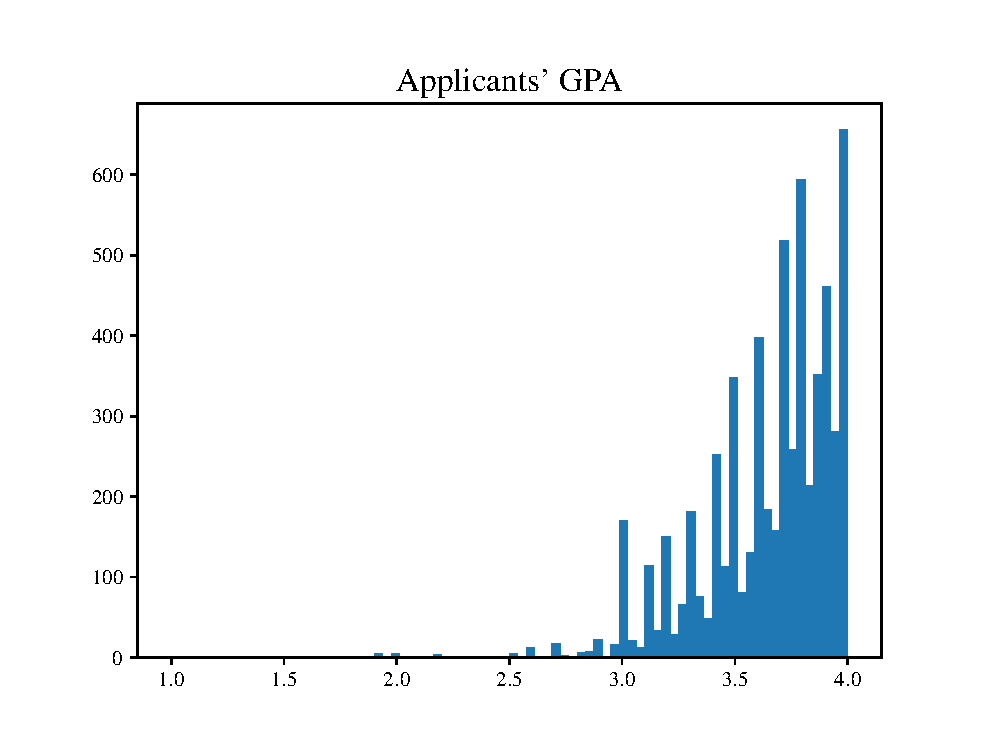
\includegraphics[width=\textwidth]{gpa.eps}
	\caption{Histogram of Applicants' GPA.}
    \end{subfigure}%
    \begin{subfigure}{.5\linewidth}\centering
	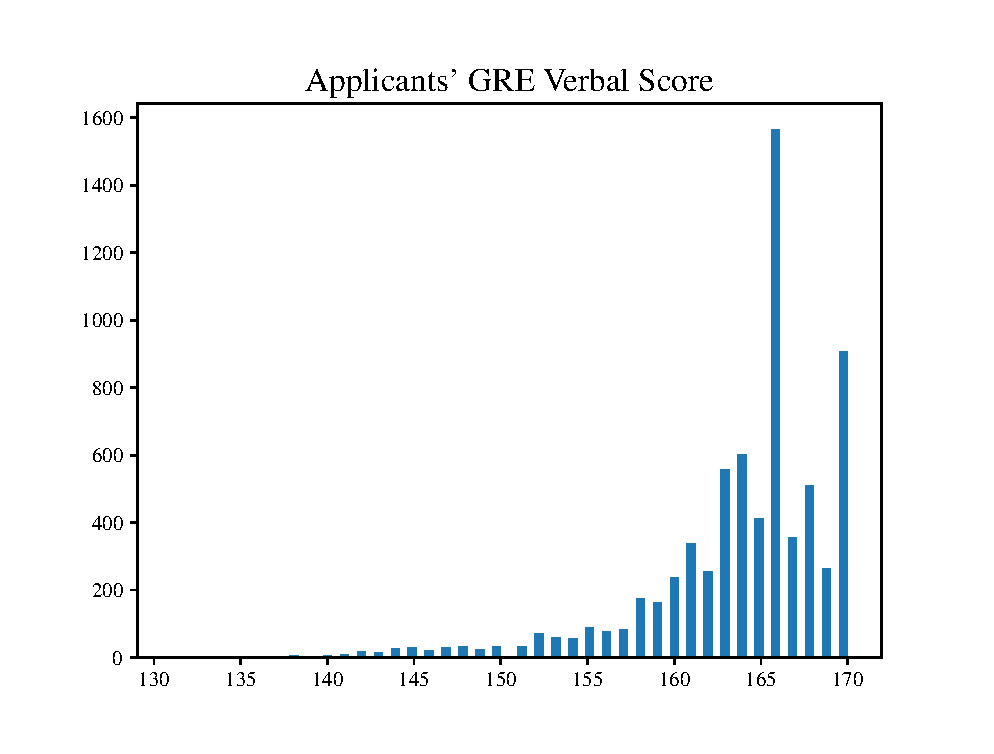
\includegraphics[width=\textwidth]{gre.eps}
	\caption{Histogram of Applicants' GRE Verbal Score.}
    \end{subfigure}
    \begin{subfigure}{.5\linewidth}\centering
	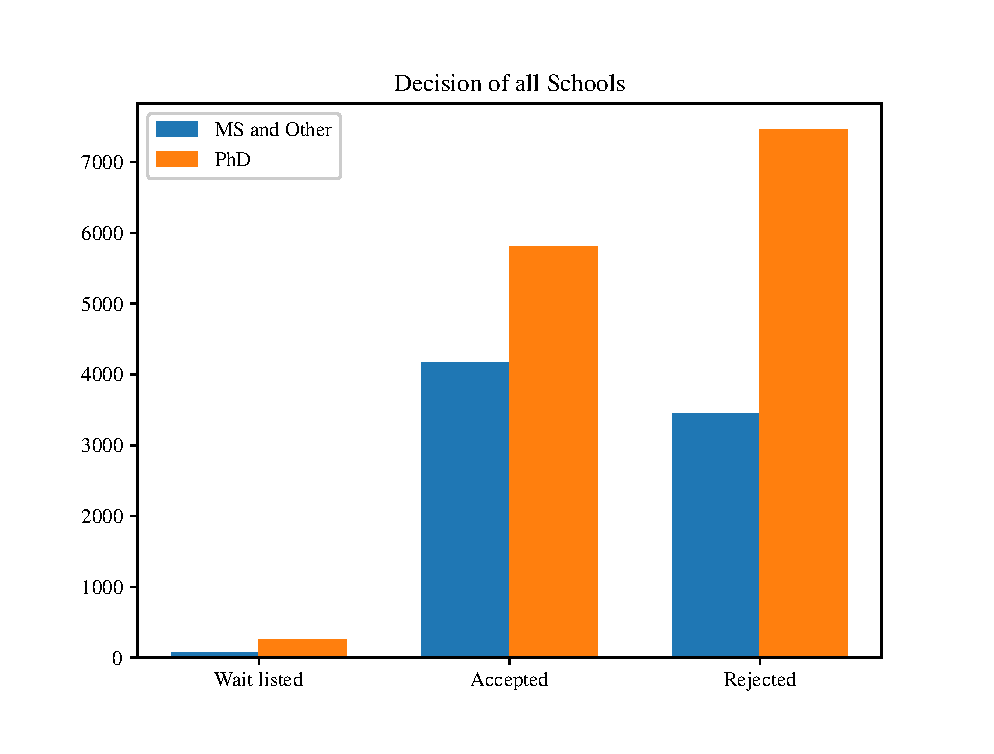
\includegraphics[width=\textwidth]{all_decision.eps}
	\caption{Overall Decisions.}
    \end{subfigure}%
    \begin{subfigure}{.5\linewidth}\centering
	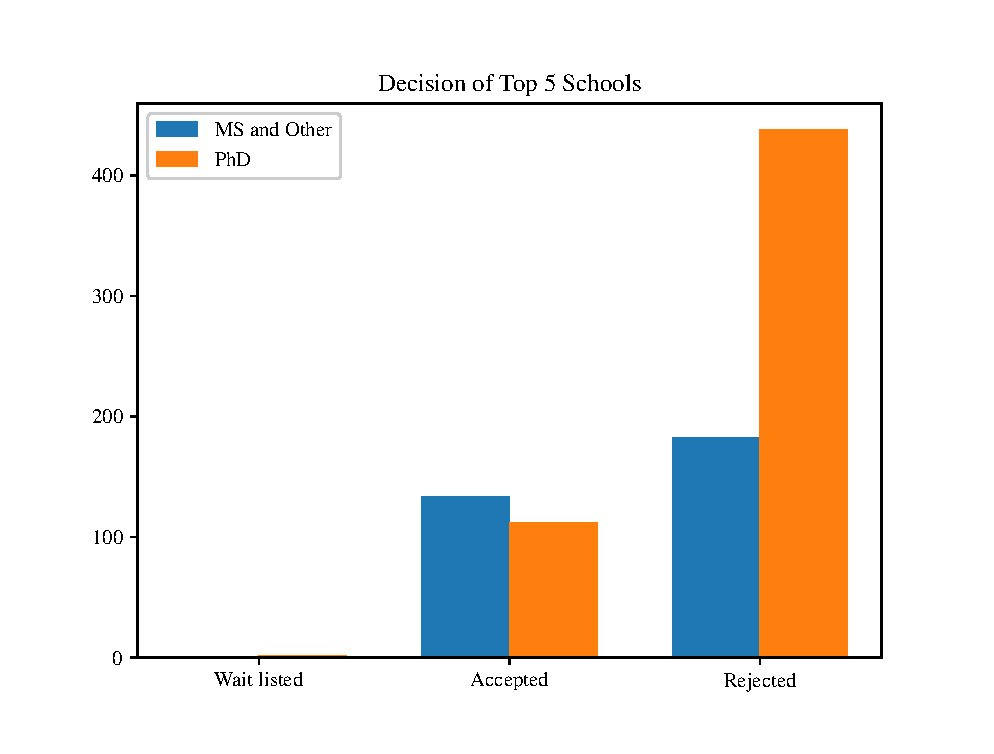
\includegraphics[width=\textwidth]{top5_decision.eps}
	\caption{Decisions from Top 5 Schools.}
    \end{subfigure}%
    \caption{Histograms of Selected Covariates.}  \label{fig:dataset}
\end{figure}

	\begin{table}[htpb]
	    \centering
	    \begin{tabular}{cccc}
		Institution & Program (Season) & Decision \& Date & Status \\\hline\hline
		\emph{Stanford University} & CS Masters (F18) & Rejected via E-mail on 16 March 2018 & I \\
		\multicolumn{4}{l}{Comment: \emph{I think I have no grad schools to attend next year.}}\\
		\emph{Stanford University} & CS PhD (F18) & Accepted via Phone on 7 Feb 2018 & U \\
		\multicolumn{4}{l}{Comment: \emph{Call from POI and email from student buddy. Absolutely shocked and very excited.}}\\
		\ldots\\
		\emph{UC Berkeley} & EECS PhD (F18) & Accepted via E-mail on 2 Feb 2018 & A \\
		\multicolumn{4}{l}{Comment: \emph{Accepted with nomination for university fellowship. 1 first author conference talk...}}\\ \hline\hline
	    \end{tabular}
	    \caption{Samples of \noun{GradCafe} dataset.}
	    \label{table:data_sample}
	\end{table}
	In this paper, we collect data from \textbf{GradCafe}, an online
	sharing platform of graduate school admission results. The dataset
	involves the following covariates:
	\var{university}, the graduate school the applicant applied for;
	\var{degree}, one of either \var{\{MBA, MEng, MFA, MS, PhD, Other\}}, the desired degree applied for;
	\var{decision}, one of either \var{\{Accepted, Rejected, Wait Listed\}}, the application result;
	\var{gpa}, the latest Grading Point Average (GPA) the applicant possesses;
	\var{gre\_verbal}, \var{gre\_quant}, \var{gre\_writing}, standard test scores examining verbal, quantitative and writing skills;
	\var{status}, either one of \var{\{American, International, International with US Degree,
	Other\}}, dictating the status of the applicant as of the application
	\var{comments}, additional information shared by the applicant. Several
	typical entries are tabulated in \Cref{table:data_sample}.

	We augment this dataset by introducing metrics examining the prestigious of the graduate
	school. Instead of selecting from a variety of university ranking, we focus on the \noun{CSRanking},
	which is specifically tailored for CS research. To that end, we attach two more covariates per record,
	namely,
	\var{publications}, publication index, the multiplier of number of total publications with reference
	to the lowest value;
	\var{faculty}, the number of faculty members (not counting Emeritus faculties).
	We note through our data exploration, these metrics, though may seem partial at first mention,
	are consistent with the general ranking results from, for example, US News \cite{}, Times \cite{},
	to name a few.

	We preprocess the dataset to select those applications made to US universities,
	clean up invalid data, normalize the GPA on a $4.0$ scale and GRE tests
	to new scale ($170$ maximum). We also merge the categories \var{\{MBA, MEng, MFA, MS, Other\}}
	to a singleton \var{MS} as it suffices the objectives set for this paper. After these manipulations,
	we had $21209$ records from the applications ranging from $2011$ to $2015$. Noted some records
	may miss certain metrics such as GPA, in that case, our model ignore the very entries for parameter
	estimation. A short summary of the cleaned dataset is given in \Cref{table:data_summary:quant,table:data_summary:cat}. We also plot the histogram of several selected covariates in \Cref{fig:dataset}.

	\begin{table}[htpb]
	    \centering
	    \begin{tabular}{|c|c|c|c|c|c|}
		\hline
		Covariate & Available Record & Min. & Mean & Median & Max. \\\hline
		\var{gpa} & $6015$ & $1.00$ & $3.65$ & $3.70$ & $4.00$ \\\hline
		\var{gre\_verbal} & $7078$ & $130.0$ & $157.8$ & $158.0$ & $170.0$ \\\hline
		\var{gre\_quant} & $7078$ & $131.0$ & $163.9$ & $166.0$ & $170.0$ \\\hline
		\var{gre\_writing} & $6873$ & $2.00$ & $3.89$ & $4.00$ & $6.00$ \\\hline
		\var{publication} & all & $1.00$ & $6.38$ & $5.40$ & $18.10$ \\\hline
		\var{faculty} & all & $2$ & $53$ & $50$ & $152$ \\\hline
	    \end{tabular}
	    \caption{Summary for Quantitative Covariates.}
	    \label{table:data_summary:quant}
	\end{table}

	\begin{table}[htpb]
	    \centering
	    \begin{subtable}{0.2\textwidth}\centering
	    \begin{tabular}{|c|c|}
		\hline
		MS & PhD \\\hline
		7693 & 13516 \\\hline
	    \end{tabular}
		\caption{\var{degree}.}
	    \end{subtable}%
	    \begin{subtable}{0.4\textwidth}\centering
	    \begin{tabular}{|c|c|c|}
		\hline
		Accepted & Rejected & Wait Listed \\\hline
		9971 & 10912 & 326 \\\hline
	    \end{tabular}
		\caption{\var{decision}.}
	    \end{subtable}%
	    \begin{subtable}{0.4\textwidth}\centering
	    \begin{tabular}{|c|c|c|c|}
		\hline
		A & U & I & O \\\hline
		4159 & 2747 & 13546 & 219 \\\hline
	    \end{tabular}
		\caption{\var{status}.}
	    \end{subtable}
	    \caption{Summary for Categorical Covariates.}
	    \label{table:data_summary:cat}
	\end{table}



\note{A sketchy mention of the methods should suffice}


\section{Methods} \label{sec:methods}

\section{Results and Model Selection} \label{sec:results}

\section{Conclusions and Future Directions} \label{sec:conclusions}

    In this paper, we study the factors that are significant
    to the applications for CS graduate programs in the U.S.
    We remark that, the model proposed does not account for
    the representativeness of the data collected. Namely,
    the data collected may be not a representative sample
    from the unknown population; the data may be more correlated
    as intuitively, most failed applicants may wish not to share
    this experience online. For the sake of completeness,
    we remark that imposing a Bayesian model or use multilevel
    regression and postratification (MRP) \cite{} may ameliorate
    these issues, we are, nonetheless, content with this model
    in this rather introductory and casual writing.

{\small
\nocite{*}
\bibliography{report}
\bibliographystyle{alpha}
}
\ifthenelse{\equal{\final}{0}}


\end{document}
